% Temporarily allow 3 floats at the top on a page
% This needs to be set well before any figure to which this is to be applied
\setcounter{topnumber}{3}%%ALLOWLATEX%%
\setcounter{totalnumber}{4}%%ALLOWLATEX%%


\chapter{\texorpdfstring{\MPI/}{MPI} Terms and Conventions}
\label{chap:terms}
\label{sec:terms}
\label{chap:terms-2}
\label{sec:terms-2}

This chapter explains notational terms and conventions used
throughout the
\MPI/
document, some of the choices that have been made,
and the rationale behind those choices.

%%%%%%%%%%%%%%%%%%%%%%%%%%%%%%%%%%%%%%%%%%%%%%%%%%%%%%%%%%%%%%%%%%%%%%
\section{Document Notation}

\begin{rationale}
Throughout this document, the rationale for the design choices made in
the interface specification is set off in this format.  Some readers may
wish to skip these sections, while readers interested in interface design
may want to read them carefully.
\end{rationale}

\begin{users}
Throughout this document, material aimed at users and that illustrates
usage is set off in this format.  Some readers may
wish to skip these sections, while readers interested in programming in \MPI/
may want to read them carefully.
\end{users}

\begin{implementors}
Throughout this document, material that is primarily commentary to implementors
is set off in this format.  Some readers may
wish to skip these sections, while readers interested in
\MPI/ implementations may want to read them carefully.
\end{implementors}

%%%%%%%%%%%%%%%%%%%%%%%%%%%%%%%%%%%%%%%%%%%%%%%%%%%%%%%%%%%%%%%%%%%%%%
% wcs
\section{Naming Conventions}
\label{subsec:terms:naming}

In many cases \MPI/ names for C functions are of the form
\mpiskipfunc{MPI\_Class\_action\_subset}. This convention originated with \MPII/. Since \MPIII/ an
attempt has been made to standardize the names of \MPI/ functions according to
the following rules.

\begin{enumerate}
\item
In C and the Fortran \code{mpi\_f08} module, all routines associated with a particular type of \MPI/ object
should be of the form \mpiskipfunc{MPI\_Class\_action\_subset} or, if no subset
exists, of the form \mpiskipfunc{MPI\_Class\_action}.
In the Fortran \code{mpi} module and (deprecated) \code{mpif.h} file, all routines
associated with a particular type of \MPI/ object should be of the form
\mpiskipfunc{MPI\_CLASS\_ACTION\_SUBSET} or, if no subset exists, of the form
\mpiskipfunc{MPI\_CLASS\_ACTION}.

\item
If the routine is not associated with a class, the name
should be of the form \mpiskipfunc{MPI\_Action\_subset} or
\mpiskipfunc{MPI\_ACTION\_SUBSET} in C and Fortran.

\item
The names of certain actions have been standardized. In
particular, \mpitermdefni{create}\mpitermdefindex{create!in function names}
creates a new object, \mpitermdefni{get}\mpitermdefindex{get!in function names}
retrieves information about an object, \mpitermdefni{set}\mpitermdefindex{set!in function names} sets
this information, \mpitermdefni{delete}\mpitermdefindex{delete!in function names} deletes information,
\mpitermdefni{is}\mpitermdefindex{is!in function names} asks whether or not an object has a certain property.

\end{enumerate}

C and Fortran names for
some \MPI/ functions (that were defined during the \MPII/ process)
violate these rules
in several cases. The most common exceptions are the omission
of the \mpitermdefni{Class}\mpitermdefindex{class!in function names} name from the routine and the omission of
the \mpitermdefni{Action}\mpitermdefindex{action!in function names} where one can be inferred.


%%%%%%%%%%%%%%%%%%%%%%%%%%%%%%%%%%%%%%%%%%%%%%%%%%%%%%%%%%%%%%%%%%%%%%
\section{Procedure Specification}
\mpitermtitleindex{procedure specification}
\mpitermtitleindex{procedure!specification}
\label{terms:procedure-specification}

\MPI/ procedures are specified using a language-independent notation.
The arguments of procedure calls are marked as \IN, \OUT, or
\INOUT.  The meanings of these are:
\begin{description}
\item[\IN:]
  the call may use the input value but does not update the
  argument from the perspective of the caller at any time during the call's execution,
\item[\OUT:]
  the call may update the argument but does not use its input value,
\item[\INOUT:]
  the call may both use and update the argument.
\end{description}

There is one special case---if an argument is a handle to
an opaque object (these terms are defined in
Section~\ref{terms:opaque-objects}), and the
object is updated by the procedure call, then the argument is marked
\INOUT\ or
\OUT.  It is marked this way even though the handle itself is not
modified---we use the
\INOUT\ or
\OUT\ attribute to denote that what the
handle \emph{references} is updated.

\begin{rationale}
The definition of \MPI/ tries to avoid, to the largest possible extent,
the use of \INOUT\ arguments, because such use is error-prone,
especially for scalar arguments.
\end{rationale}

\MPI/'s use of \IN, \OUT, and \INOUT\ is intended
to indicate to the user how an argument is
to be used, but
does not provide a rigorous classification that can be translated
directly into
all
language bindings (e.g., \code{INTENT} in Fortran 90 bindings
or \code{const} in C bindings). For instance, the ``constant''
\mpiconst{MPI\_BOTTOM} can usually be passed to \OUT\ buffer
arguments. Similarly, \mpiconst{MPI\_STATUS\_IGNORE} can be passed as the
\OUT\ status argument.

A common occurrence for \MPI/ functions is an argument that is used as
\IN{}
by some processes and \OUT\ by other processes. Such
an argument is, syntactically, an \INOUT\ argument and is marked as
such, although, semantically, it is not used in one call both for
input and for output on a single process.

Another frequent situation arises when an argument value is needed only by
a subset of the processes.  When an argument is not significant at a
process then an arbitrary value can be passed as an argument.

\begin{users}
Note that the programmer is still responsible for avoiding undefined behavior in the host language by not passing uninitialized values to \mpi/ procedure calls.
\end{users}

Unless specified otherwise, an argument of type \OUT\ or type
\INOUT\ cannot be aliased with any other argument passed to an
\MPI/ procedure.  An example of argument aliasing in C appears below.
If we define a C procedure like this,
%%HEADER
%%LANG: C
%%ENDHEADER
\begin{lstlisting}[language=C]
void copyIntBuffer(int *pin, int *pout, int len)
{   int i;
    for (i=0; i<len; ++i) *pout++ = *pin++;
}
\end{lstlisting}
then a call to it in the following code fragment has aliased arguments.
%%HEADER
%%LANG: C
%%FRAGMENT
%%DECL: void copyIntBuffer(int *, int *, int);
%%ENDHEADER
\begin{lstlisting}[language=C]
int a[10];
copyIntBuffer(a, a+3, 7);
\end{lstlisting}
Although the C language allows this, such usage of \MPI/ procedures is
forbidden unless otherwise specified.  Note that Fortran prohibits
aliasing of arguments.

All \MPI/ functions are first specified in the language-independent
notation.  Immediately below this, language dependent bindings follow:
\begin{itemize}
\item The ISO C version(s) of the function.
\item The Fortran version(s) used with \code{USE mpi\_f08}.
\item The Fortran version of the same
      function used with \code{USE mpi} or (deprecated) \code{INCLUDE 'mpif.h'}.
\end{itemize}
Some \MPI/ procedures have two interfaces for a given language support;
see Sections~\ref{subsec:displacement} and~\ref{subsec:count}.

An exception is \sectionref{sec:mpit} ``The \MPI/ Tool Information Interface'',
which only provides ISO C interfaces.

``Fortran'' in this document refers to Fortran 90 or later; see
\sectionref{subsec:binding}.

The words function, routine, procedure, procedure call, and call are often used as synonyms within this standard.

%%%%%%%%%%%%%%%%%%%%%%%%%%%%%%%%%%%%%%%%%%%%%%%%%%%%%%%%%%%%%%%%%%%%%%
\section{Semantic Terms}
\mpitermtitleindex{semantics}
\mpitermtitleindex{semantics!terms}
\label{terms:semantic}

When discussing \MPI/ procedures the following semantic terms are
used.  The term \textbf{message data buffer} refers to the send/receive
buffer used in a communication procedure.  The term
\textbf{file data buffer} refers to the data buffers used by \MPI/ I/O
procedures. In this section we use the term \textbf{data buffer} and
depending on the \MPI/ procedure it will refer to message data buffer
or file data buffer.
\annexref{sec:lang:semantics:summary} shows how the terms defined in
this section apply to all operation-related \MPI/ procedures.

\subsection{\texorpdfstring{\MPI/}{MPI} Operations}
\mpitermtitleindex{MPI operation@\MPI/ operation}
\mpitermtitleindex{operation}
\mpitermtitleindex{semantics!operation}
\mpitermtitleindex{operation!semantics}
\label{subsec:operations}
\begin{description}
\item[\mpitermdefni{\MPI/ operation}:]
An \MPI/ operation is a sequence of steps performed by the \MPI/
library to establish and enable data transfer and/or synchronization.
It consists of four stages\mpitermdefindex{operation!stage}\mpitermdefindex{stage}:
initialization, starting, completion, and freeing, and it is implemented
as a set of one or more \MPI/ procedures,
see Section~\ref{subsec:procedures}.

\begin{description}
\item[\mpitermdefni{Initialization}]\mpitermdefindex{initialization
    stage}\mpitermdefindex{stage!initialization}\mpitermdefindex{operation!stage!initialization} hands over the
  argument list to the operation but not the content of the data
  buffers, if any.  The specification of an operation may state that
  array arguments must not be changed until the operation is freed.

\item[\mpitermdefni{Starting}]\mpitermdefindex{starting
    stage}\mpitermdefindex{stage!starting}\mpitermdefindex{operation!stage!starting} hands over control of
  the data buffers, if any, to the associated operation.

Note that \mpitermdef{initiation} refers to the combination of the
initialization and starting stages.

\item[\mpitermdefni{Completion}]\mpitermdefindex{completion
    stage}\mpitermdefindex{stage!completion}\mpitermdefindex{operation!stage!completion} returns control of the
  content of the data buffers and indicates that output buffers and
  arguments, if any, have been updated.

  Note that an \MPI/ operation is
  \mpitermdefni{complete}\mpitermdefindex{complete
    operation}\mpitermdefindex{operation!complete} when the \MPI/
  procedure implementing the completion stage returns.

\item[\mpitermdefni{Freeing}]\mpitermdefindex{freeing
    stage}\mpitermdefindex{stage!freeing}\mpitermdefindex{operation!stage!freeing} returns control of the rest
  of the argument list (e.g., the data buffer address and array
  arguments).
\end{description}

% Explanation to Forum members:
% -----------------------------
% We choose initialization and completion (nouns) intentionally
% instead of initializing and completing because the ...ing
% forms (gerunds serving as nouns) are only rarely used from
% Chapters 2 through the end in existing MPI standard documents.
% However, where these appear, their meaning is identical to their
% corresponding parts of speech.
\end{description}

\noindent \MPI/ operations are available in one or more of these forms:
blocking, nonblocking, and persistent.

\begin{description}
\item[\mpitermdefni{Blocking operation}:]\mpitermdefindex{blocking operation}\mpitermdefindex{operation!blocking}
For a \textbf{blocking operation}, all four stages are combined in a
single procedure call (as shown in
Figure~\ref{fig:state-diagram-blocking} and defined in
Section~\ref{subsec:procedures}).


\begin{figure}[t]
  \centerline{%
    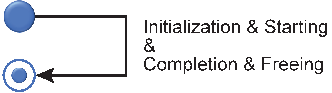
\includegraphics[width=2in]{figures/blocking-state-diagram.pdf}}
    \caption{State transition diagram for blocking operations}
    \label{fig:state-diagram-blocking}
\end{figure}

\item[\mpitermdefni{Nonblocking operation}:]\mpitermdefindex{nonblocking operation}\mpitermdefindex{operation!nonblocking}
For a \textbf{nonblocking operation},
the initialization and starting stages are combined into a single nonblocking
procedure call and the completion and freeing stages are combined into a
separate, single procedure call, which can be blocking or nonblocking
(as shown in Figure~\ref{fig:state-diagram-nonblocking} and defined in
Section~\ref{subsec:procedures}).

\begin{figure}[t]
\centerline{%
   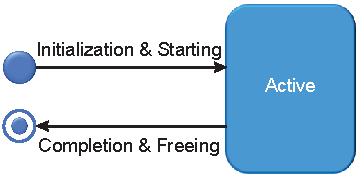
\includegraphics[width=2in]{figures/nonblocking-state-diagram.pdf}}
    \caption{State transition diagram for nonblocking operations}
   \label{fig:state-diagram-nonblocking}
\end{figure}

\item[\mpitermdefni{Persistent operation}:]\mpitermdefindex{persistent operation}\mpitermdefindex{operation!persistent}
For a \textbf{persistent operation}, there is a separate procedure for each of the four stages
(as shown in Figure~\ref{fig:state-diagram-persistent} and defined in
Section~\ref{subsec:procedures}).
Each of these procedures may be blocking or nonblocking.

For a partitioned send operation\mpitermdefindex{operation!partitioned send},
an additional call to activate each partition of the send buffer (see Section~\ref{sec:part_comm_init})
is required to finish the starting stage.
For a partitioned receive operation\mpitermdefindex{operation!partitioned receive},
before the operation is complete the user is allowed to access a partition of the output buffer after verifying that it has arrived (see
Section~\ref{subsec:part-commend}).

\begin{figure}[t]
    \centerline{%
    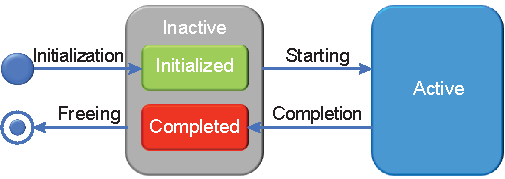
\includegraphics[width=3.0in]{figures/persistent-state-diagram.pdf}}
    \caption{State transition diagram for persistent operations}
    \label{fig:state-diagram-persistent}
\end{figure}

\end{description}

These four stages lead to the \mpitermdefni{operation states}\mpitermdefindex{operation!state}\mpitermdefindex{state!operation}
\mpitermdefni{initialized}\mpitermdefindex{initialized operation state}\mpitermdefindex{operation!state!initialized}\mpitermdefindex{state!operation!initialized},
\mpitermdefni{started}\mpitermdefindex{started operation state}\mpitermdefindex{operation!state!started}\mpitermdefindex{state!operation!started},
\mpitermdefni{complete}\mpitermdefindex{complete operation state}\mpitermdefindex{operation!state!complete}\mpitermdefindex{state!operation!complete}, and
% Comment for the MPI forum: Here we use "complete" instead of "completed" because at the definition
%                            of the "completion stage", the state "complete" was already defined
%                            in MPI-4.0. And there, we have 283x "complete" and 138x "completed".
\mpitermdefni{freed}\mpitermdefindex{freed operation state}\mpitermdefindex{operation!state!freed}\mpitermdefindex{state!operation!freed}.
A \mpitermni{started operation} is also named
\mpitermdefni{active}\mpitermdefindex{active!operation state}\mpitermdefindex{operation!state!active}\mpitermdefindex{state!operation!active},
and the states \mpitermni{initialized} and \mpitermni{complete} are also named
\mpitermdefni{inactive}\mpitermdefindex{inactive!operation state}\mpitermdefindex{operation!state!inactive}\mpitermdefindex{state!operation!inactive}.

\mpitermni{Active} communication and I/O operations are also named
\mpitermdefni{pending}\mpitermdefindex{pending (communication) operation}\mpitermdefindex{pending I/O operation}\mpitermdefindex{communication!pending}\mpitermdefindex{operation!pending} operations.
Note that a \mpitermni{pending} operation can be
a nonblocking or persistent operation that is started and not yet complete
(even if the request handle has been freed),
or a blocking operation that is not yet complete, such as a receive operation
that is waiting for a message to be received.

% The following text is introducing a new set of topics - (non)collective
\medskip %%ALLOWLATEX%%

Additionally, an \MPI/ operation can be collective or noncollective.

\begin{description}
\item[\mpitermdefni{Collective operation}:]\mpitermdefindex{collective operation}\mpitermdefindex{operation!collective}
A \textbf{collective operation} is a set of related operations, one per \MPI/ process in a group
or groups of \MPI/ processes. For collective operations the completion
stage may or may not finish before all processes in the group have
started the operation.

Collective \MPI/ operations are also available as blocking, nonblocking, or persistent operations.

\item[\mpitermdefni{Noncollective operation}:]\mpitermdefindex{noncollective operation}\mpitermdefindex{operation!noncollective}
\textbf{Noncollective operations} are defined as operations that are not collective.
\end{description}


Many \MPI/ operations coordinate activities at multiple \MPI/ processes:
the semantics of such an operation require one or more other specific semantically-related operations to be \mpitermni{started}
before it is guaranteed that the operation can transition to the \mpitermni{complete} operation state.
For example, a receive operation requires a related send operation to be started before the receive can complete;
or a collective operation might not complete before such operations are also started in all \MPI/ processes of the respective group.

\begin{description}
%% Some possible additional terms are kept as comment for the case that a future MPI forum may want to add more details.
%% For MPI-4.1 it is decided to only standardize "enabled" as an abbreviation of "fully enabled" of the original list.
% \item[\mpitermdefni{Totally enabled}]\mpitermdefindex{totally enabled operation state}\mpitermdefindex{enabled operation state!totally}\mpitermdefindex{state!operation!totally enabled}\mpitermdefindex{operation!state!totally enabled}
%    An \MPI/ operation is \mpitermdefni{totally enabled} at a particular \MPI/ process when all specific semantically-related operations
%    have been started.
%% enabled = fully enabled, if one of the other terms may be added
\item[\mpitermdefni{Enabled}:]\mpitermdefindex{enabled operation state}\mpitermdefindex{state!operation!enabled}\mpitermdefindex{operation!state!enabled}
    An \MPI/ operation is \mpitermdefni{enabled} at a particular \MPI/ process when all specific semantically-related operations
    required to guarantee completion at that \MPI/ process have been started.
%% possible additional term:
% \item[\mpitermdefni{Partially enabled}]\mpitermdefindex{partially enabled operation state}\mpitermdefindex{state!operation!partially enabled}\mpitermdefindex{operation!state!partially enabled}
%     An \MPI/ operation is \mpitermdefni{partially enabled} when at least one specific semantically-related operation
%     required to guarantee completion has been started.
% \item[\mpitermdefni{Sufficiently enabled}]\mpitermdefindex{sufficiently enabled operation state}\mpitermdefindex{enabled operation state!sufficiently}\mpitermdefindex{state!operation!sufficiently enabled}\mpitermdefindex{operation!state!sufficiently enabled}
%    An \MPI/ operation is \mpitermdefni{sufficiently enabled} at a particular \MPI/ process when all specific semantically-related operations
%    needed to guarantee completion at that particular \MPI/ process with the currently used \MPI/ implementation
%    have been started.
\end{description}

\begin{rationale}
\MPI/ implementations may include optimizations (for example, automatic buffering) that allow
an \MPI/ operation to complete before it is enabled.
% In that case, sufficiently enabled is different from fully and totally enabled.
\end{rationale}

Some \MPI/ operations are \mpitermdef{a priori enabled}\mpitermdefindex{enabled operation state!a priori}\mpitermdefindex{state!operation!enabled a priori}\mpitermdefindex{operation!state!enabled a priori},
i.e., they do not require any other specific semantically-related operation for completion.
For example, a buffered send operation completes independently of the related receive operation.

% An \MPI/ operation cannot complete until it is \mpitermni{sufficiently enabled}.
Once an \MPI/ operation is \mpitermni{enabled}, the operation must eventually complete.
% In most cases, \mpitermni{fully enabled} operations are also \mpitermni{totally enabled};
% an exception is, for example, the buffered send operation.
% If an \MPI/ operation is \mpitermni{partially enabled} and not yet started then it must eventually be started
% or the enabling operation(s) must be \mpitermni{cancelled}\mpitermindex{cancel} if this is possible.
An operation may already be enabled before it is started.
For example, a receive operation is already enabled
if it is started after the matching send operation was started.

\begin{rationale}
The definition of an operation $A$ being \mpitermni{enabled} is asymmetric:
\mpitermni{enabled} includes that all specific semantically-related operations $A'_i$ required to guarantee completion have been started,
but does not include that the operation $A$ itself is already started.

Examples:
\begin{itemize}
\item A receive is enabled exactly when the related send is started.
\item A standard mode send operation is enabled exactly when the related receive is started.
If an \MPI/ implementation chooses to use internal buffering, the send operation may be already
completed
% instead of completed:  (i.e., a priori) sufficiently enabled
before it is enabled, i.e., the receive is started.
\item A synchronous mode send operation is enabled exactly when the related receive is started
and must not complete before it is enabled.
\item A buffered mode send operation is a priori enabled.
% It is totally enabled when the related receive is started.
\item A ready mode send can be started only when it is already enabled, i.e., the related receive is started.
\item For a collective broadcast, the operation at a particular \MPI/ process is enabled exactly
      when all other \MPI/ processes in the group have started their related broadcast operation.
\end{itemize}

Specifically, for the set of related operations on a group of \MPI/ processes that constitute a collective operation that may synchronize,
the operation on a particular \MPI/ process $p$ is enabled when all other \MPI/ processes $p_i \neq p$ in the group
have started their related operation, while the operation on $p$ need not have started yet.
\end{rationale}

\subsection{\texorpdfstring{\MPI/}{MPI} Procedures}
\mpitermtitleindex{MPI procedure@\MPI/ procedure}
\mpitermtitleindex{procedure}
\mpitermtitleindex{semantics!procedure}
\mpitermtitleindex{procedure!semantics}
\label{subsec:procedures}
All \MPI/ procedures can either be \mpiterm{local} or \mpiterm{nonlocal}---defined as follows:
\begin{description}
\item[\mpitermdefni{Nonlocal procedure}:]\mpitermdefindex{nonlocal procedure}\mpitermdefindex{procedure!nonlocal}
An \MPI/ procedure is \mpitermdef{nonlocal} if returning may require, during its execution,
some specific semantically-related \MPI/ procedure to be called on another \MPI/ process.

\item[\mpitermdefni{Local procedure}:]\mpitermdefindex{local procedure}\mpitermdefindex{procedure!local}
An \MPI/ procedure is \mpitermdef{local} if it is not \mpiterm{nonlocal}.
\end{description}

An \MPI/ operation is implemented as a set of one or more \MPI/
procedures.
An \MPI/ \mpitermdefni{operation-related procedure}\mpitermdefindex{operation!operation-related}\mpitermdefindex{procedure!operation-related}
implements at least a part of a stage
of an \MPI/ operation as described in Section~\ref{subsec:operations}.
An \MPI/ operation-related procedure may also implement one or more stages of one or several \MPI/ operations.
In certain cases, more than one \MPI/ operation-related procedure may be
needed to implement a single stage.

There are also other \MPI/ procedures that do not
implement any stage of any \MPI/ operation.

The semantics of \MPI/ operation-related procedures are described using two
orthogonal (independent) concepts: completeness (depends on which
stages are included) and locality.  Such procedures can be either
incomplete, or completing, or freeing, or completing and freeing based
on the status of the associated operation at the time the procedure
returns.
Also, all such procedures can be described as either blocking or nonblocking,
but these latter two terms refer to combinations of the completeness
and locality concepts. Additionally, all \MPI/ operation-related procedures can be
collective or noncollective.

% The following text is introducing a new set of properties
\medskip %%ALLOWLATEX%%

The following are properties of \MPI/ operation-related procedures:
\begin{description}
\item[\mpitermdefni{Initialization procedure}:]\mpitermdefindex{initialization procedure}\mpitermdefindex{procedure!initialization}
An \MPI/ procedure is an \textbf{initialization procedure} if return from the
procedure indicates that the associated operation has completed its
initialization stage, which implies that the user has handed over
control of the argument list (but not contents of the data buffers) to
\MPI/.
The user is still allowed to read or modify the contents of the data buffers.
If an initializing procedure is not also the freeing procedure of the associated
operation (see below) then the user is not permitted to deallocate
the data buffers or to modify the array arguments.

\item[\mpitermdefni{Starting procedure}:]\mpitermdefindex{starting procedure}\mpitermdefindex{procedure!starting}
An \MPI/ procedure is a \textbf{starting procedure} if return from the
procedure indicates that the associated operation has completed its
starting stage, which implies that the user has handed over control of
the data buffers to \MPI/.
If a starting procedure is not also a completing procedure of the
associated operation (see below) then the user is not permitted to
modify input data buffers or to read output data buffers.

\item[\mpitermdefni{Initiation procedure}:]\mpitermdefindex{initiation procedure}\mpitermdefindex{procedure!initiation}
An \MPI/ procedure is an \textbf{initiation procedure} if return from the
procedure indicates that both the initialization and
the starting stage have completed, which implies
control of the entire argument list is handed over to \MPI/.

\item[\mpitermdefni{Completing procedure}:]\mpitermdefindex{completing procedure}\mpitermdefindex{procedure!completing}\mpitermdefindex{completing}
An \MPI/ procedure is called \textbf{completing} if return from the
procedure indicates that at least one associated operation has
finished its completion stage, which implies that the user can rely on
the content of the output data buffers and modify the content of input
and output data buffers of such operation(s). If a completing procedure is not also a
freeing procedure (see below) then the user is not permitted to
deallocate the data buffers or to modify the array
arguments.

\item[\mpitermdefni{Incomplete procedure}:]\mpitermdefindex{incomplete procedure}\mpitermdefindex{procedure!incomplete}\mpitermdefindex{incomplete}
An \MPI/ procedure is called \textbf{incomplete} if it
is not a completing procedure.

\item[\mpitermdefni{Freeing procedure}:]\mpitermdefindex{freeing procedure}\mpitermdefindex{procedure!freeing}
An \MPI/ procedure is \textbf{freeing} if return from the procedure
indicates that at least one associated operation has finished its freeing
stage, which implies that the user can reuse all parameters specified
when initializing such associated operation(s).
\end{description}

\begin{description}
\item[\mpitermdefni{Nonblocking procedure}:]\mpitermdefindex{nonblocking procedure}\mpitermdefindex{procedure!nonblocking}\mpitermdefindex{nonblocking}
An \MPI/ procedure is \textbf{nonblocking} if it is incomplete and
local.

\item[\mpitermdefni{Blocking procedure}:]\mpitermdefindex{blocking procedure}\mpitermdefindex{procedure!blocking}\mpitermdefindex{blocking}
An \MPI/ procedure is \textbf{blocking} if it is not nonblocking.
\end{description}

\begin{users}
Note that for operation-related \MPI/ procedures, in most cases
incomplete procedures are local and completing procedures are nonlocal.
Exceptions are noted where such procedures are defined.
In many cases an additional prefix
letter \mpicode{I} as an abbreviation of the words \mpitermdef{incomplete}\mpitermindex{procedure!incomplete}
and \mpitermdef{immediate}\mpitermdefindex{procedure!immediate} marks nonblocking procedures in the procedure name.

\noindent Some categorization examples are listed below.

\noindent Nonblocking procedures:
\begin{itemize}
\item incomplete and local: \mpifunc{MPI\_ISEND}, \mpifunc{MPI\_IRECV},  \mpifunc{MPI\_IBCAST},
\mpifunc{MPI\_IMPROBE}, \mpifunc{MPI\_SEND\_INIT}, \mpifunc{MPI\_RECV\_INIT}, \ldots
\end{itemize}
\noindent Blocking procedures:
\begin{itemize}
\item completing and nonlocal: \mpifunc{MPI\_SEND}, \mpifunc{MPI\_RECV}, \mpifunc{MPI\_BCAST}, \ldots
\item incomplete and nonlocal: \mpifunc{MPI\_MPROBE}, \mpifunc{MPI\_BCAST\_INIT}, \ldots,
\mpifuncindex{MPI\_FILE\_READ\_AT\_ALL\_BEGIN}%
\mpifuncindex{MPI\_FILE\_READ\_ALL\_BEGIN}%
\mpifuncindex{MPI\_FILE\_READ\_ORDERED\_BEGIN}%
\mpifuncindex{MPI\_FILE\_WRITE\_AT\_ALL\_BEGIN}%
\mpifuncindex{MPI\_FILE\_WRITE\_ALL\_BEGIN}%
\mpifuncindex{MPI\_FILE\_WRITE\_ORDERED\_BEGIN}%
\mpiskipfunc{MPI\_FILE\_\{READ$|$WRITE\}\_\{AT\_ALL$|$ALL$|$ORDERED\}\_BEGIN}.
\item completing and local: \mpifunc{MPI\_BSEND}, \mpifunc{MPI\_RSEND}, \mpifunc{MPI\_MRECV}.
\end{itemize}
\noindent \MPI/ procedures that are not \MPI/ operation-related:
\begin{itemize}
\item
\mpifunc{MPI\_COMM\_RANK}, \mpifunc{MPI\_WTIME}, \mpifunc{MPI\_PROBE},  \mpifunc{MPI\_IPROBE}, \ldots
\end{itemize}
\end{users}

\begin{description}
\item[\mpitermdefni{Collective procedure}:]\mpitermdefindex{collective procedure}\mpitermdefindex{procedure!collective}\mpitermdefindex{collective}
An \MPI/ procedure is \textbf{collective} if all processes in a group or groups of \MPI/ processes need to invoke the procedure.

Initialization procedures of collective operations over the same
process group must be executed in the same order by all members of the
process group.

%\item[\mpitermdefni{Synchronizing procedure}]\mpitermdefindex{synchronizing procedure}\mpitermdefindex{procedure!synchronizing}
An \MPI/ collective procedure is \textbf{synchronizing}\mpitermdefindex{synchronizing procedure}\mpitermdefindex{procedure!synchronizing} if it will
only return once all processes in the associated group or groups of \MPI/ processes have called the
appropriate matching \MPI/ procedure.

The initiation procedures for nonblocking collective operations and
the starting procedures for persistent collective operations are local
and shall not be synchronizing.

All other procedures for collective operations,
such as for blocking collective operations and the
initialization procedures for persistent collective operations, may or
may not be synchronizing.

\begin{users}
Calling any synchronizing function is erroneous when there is no possibility of
corresponding calls at all other processes in the associated process
group.

Waiting for completion of any collective operation is erroneous when there is no possibility
that all other processes in the associated group will be able to start
the corresponding operation.
\end{users}

\item[\mpitermdefni{Noncollective procedure}:]\mpitermdefindex{noncollective procedure}\mpitermdefindex{procedure!noncollective}
Noncollective procedures are defined as procedures that are not collective.
\end{description}

The definition of
\mpitermdefni{local}\mpitermdefindex{local procedure!call, under constraint}\mpitermdefindex{procedure!local!call, under constraint}
and
\mpitermdefni{nonlocal}\mpitermdefindex{nonlocal procedure!call, under constraint}\mpitermdefindex{procedure!nonlocal!call, under constraint}
\MPI/ procedures
can also be applied to a specific procedure invocation or to procedure calls \mpitermdefni{under certain constraints}.
For example, a call to a completing receive procedure that happens after the related
send operation was already started may be described as local, even though the completing receive procedure without the constraint is nonlocal.
More generally, a call to any completing procedure that happens after the operation was already
\mpitermni{enabled}\mpitermindex{enabled operation state}\mpitermindex{state!operation!enabled}\mpitermindex{operation!state!enabled}
is local, even if the completing procedure without the constraint is nonlocal.
Another example, a call to a blocking collective procedure using a process group of size one is local, even if the blocking collective procedure without the constraint is nonlocal.

\subsection{\texorpdfstring{\MPI/}{MPI} Datatypes}
\mpitermtitleindex{MPI datatype@\MPI/ datatype}
\mpitermtitleindex{datatype}
\label{terms:datatypes}
For datatypes, the following terms are defined:

\begin{description}
\item[\mpitermdefni{predefined}\mpitermdefindex{predefined datatype}:]\mpitermdefindex{datatype!predefined}
A predefined datatype is a datatype with a predefined (constant) name
(such as \mpidtype{MPI\_INT}, \mpidtype{MPI\_FLOAT\_INT}, or \mpidtype{MPI\_PACKED})
or a datatype constructed with \mpifunc{MPI\_TYPE\_CREATE\_F90\_INTEGER},
\mpifunc{MPI\_TYPE\_CREATE\_F90\_REAL}, or
\mpifunc{MPI\_TYPE\_CREATE\_F90\_COMPLEX}.  The former are \mpitermdefni{named}\mpitermdefindex{named datatype}\mpitermdefindex{datatype!named}
whereas the latter are \mpitermdefni{unnamed}\mpitermdefindex{unnamed datatype}\mpitermdefindex{datatype!unnamed}.
\item[\mpitermdefni{derived}\mpitermdefindex{derived datatype}:]\mpitermdefindex{datatype!derived}
A derived datatype is any datatype that is not predefined.
\item[\mpitermdefni{portable}\mpitermdefindex{portable datatype}:]\mpitermdefindex{datatype!portable}
A datatype is portable if it is a predefined datatype, or it is derived
from a portable datatype using only the type constructors
\mpifunc{MPI\_TYPE\_CONTIGUOUS}, \mpifunc{MPI\_TYPE\_VECTOR},
\mpifunc{MPI\_TYPE\_INDEXED}, \flushline % To force fit in margin
\mpifunc{MPI\_TYPE\_CREATE\_INDEXED\_BLOCK},
\mpifunc{MPI\_TYPE\_CREATE\_SUBARRAY}, \mpifunc{MPI\_TYPE\_DUP}, and
\mpifunc{MPI\_TYPE\_CREATE\_DARRAY}.
Such a datatype is portable because all displacements in the datatype
are in terms of extents of one predefined datatype.  Therefore, if such a
datatype fits a data layout in one memory, it will fit the
corresponding data layout in another memory, if the same declarations
were used, even if the two systems have different architectures.  On
the other hand, if a datatype was constructed using
\mpifunc{MPI\_TYPE\_CREATE\_HINDEXED},
\mpifunc{MPI\_TYPE\_CREATE\_HINDEXED\_BLOCK},
\mpifunc{MPI\_TYPE\_CREATE\_HVECTOR} or
\mpifunc{MPI\_TYPE\_CREATE\_STRUCT}, then the datatype contains explicit byte
displacements (e.g., providing padding to meet alignment restrictions).
These displacements are unlikely to be chosen correctly if they fit
data layout on one memory, but are used for data layouts on another
process, running on a processor with a different architecture.
\item[\mpitermdefni{equivalent}\mpitermdefindex{equivalent datatypes}:]\mpitermdefindex{datatype!equivalent}
Two datatypes are equivalent if they appear to have been created with
the same sequence of calls (and arguments) and thus have the same
typemap.  Two equivalent datatypes do not necessarily have the same
cached attributes or the same names.
\end{description}

%%%%%%%%%%%%%%%%%%%%%%%%%%%%%%%%%%%%%%%%%%%%%%%%%%%%%%%%%%%%%%%%%%%%%%
\section{Datatypes}

%%%%%%%%%%%%%%%%%%%%%%%%%%%%%%%%%%%%%%%%%%%%%%%%%%%%%%%%%%%%%%%%%%%%%%
\subsection{Opaque Objects}
\mpitermtitleindex{opaque objects}
\label{terms:opaque-objects}

\MPI/ manages \mpitermdef{system memory}\mpitermdefindex{memory!system} that is used for buffering
messages and for storing internal representations of various \MPI/ objects
such as groups, communicators, datatypes, etc.
This memory is not directly accessible to the user, and objects stored
there are \mpitermdefni{opaque}: their size and shape is not visible to the
user.  Opaque objects are accessed via \mpitermdef{handles}, which exist in
user space.  \MPI/ procedures that operate on opaque objects are
passed handle arguments to access these objects.
In addition to their use by \MPI/ calls for object access, handles can
participate in assignments and comparisons.

In Fortran with \code{USE mpi} or (deprecated) \code{INCLUDE 'mpif.h'},
all handles have type \ftype{INTEGER}.
In Fortran with \code{USE mpi\_f08}, and in C, a
different handle type is defined for each category of objects.
With Fortran \code{USE mpi\_f08}, the handles are defined
as Fortran \ftype{BIND(C)} derived types that consist of only
one element \ftype{INTEGER} \code{::} \code{MPI\_VAL}. The internal handle
value is identical to the Fortran \ftype{INTEGER} value
used in the \code{mpi} module and (deprecated) \code{mpif.h}.
The operators \code{.EQ.}, \code{.NE.}, \code{==} and \code{/=} are
overloaded to allow the comparison of these handles.
The type names are identical to the names in C, except
that they are not case sensitive.
For example:\cdeclindex{MPI\_Comm}\cdeclindex{MPI\_VAL}
%%HEADER
%%LANG: FORTRAN08
%%SKIP
%%ENDHEADER
\begin{lstlisting}[language={[MPI08]Fortran}]
TYPE, BIND(C) :: MPI_Comm
  INTEGER   :: MPI_VAL
END TYPE MPI_Comm
\end{lstlisting}

The C types must support the use of the assignment and equality
operators.

\begin{implementors}
In Fortran, the handle can be an index into a table of opaque objects
in a system table; in C it can be such an index or a pointer to the
object.
\end{implementors}

\begin{rationale}
Since the Fortran integer values are equivalent, applications can easily
convert \MPI/ handles between all three supported Fortran methods.  For
example, an integer communicator handle \code{COMM} can be converted directly
into an exactly equivalent \code{mpi\_f08} communicator handle named \code{comm\_f08}
by \code{comm\_f08\%MPI\_VAL=COMM}, and vice versa.
The use of the \ftype{INTEGER} defined handles and the
\ftype{BIND(C)} derived type handles is different:
Fortran 2003 (and later) define that \ftype{BIND(C)} derived types
can be used within user defined common blocks, but it is up to
the rules of the companion C compiler how many numerical storage units
are used for these \ftype{BIND(C)} derived type handles.
Most compilers use one unit for both, the \ftype{INTEGER} handles and the handles defined as
\ftype{BIND(C)} derived types.
\end{rationale}
\begin{users}
If a user wants to substitute the \code{mpi} module or the (deprecated) \code{mpif.h}
by the \code{mpi\_f08} module and the
application program stores a handle in a Fortran common block
then it is necessary to change the Fortran support method
in all application routines that use this common block,
because the number of numerical storage units of such a handle
can be different in the two modules.
\end{users}

Opaque objects are allocated and deallocated
by calls that are specific to each object type.
These are listed in the sections where the objects are described.
The calls accept a handle argument of matching type.
In an allocate call this is an \OUT\ argument that
returns a valid reference to the object.
In a call to deallocate this is an \INOUT\ argument that returns
with an ``invalid handle'' value.
\MPI/ provides an ``invalid handle'' constant
for each object type.  Comparisons to this constant are used to test for
validity of the handle.

A call to a deallocate routine invalidates the handle and marks the
object for deallocation.  The object is not accessible to the user
after the call.  However, \MPI/ need not deallocate the object
immediately.  Any operation \mpitermni{pending}\mpitermindex{pending (communication) operation}\mpitermindex{communication!pending}\mpitermindex{operation!pending} (at the time of the deallocate)
and \mpitermni{decoupled \MPI/ activity}\mpitermindex{decoupled MPI activities@decoupled \MPI/ activities} (see \sectionref{subsec:terms:progress})
that involves this object will complete normally; the object will be
deallocated afterwards.

An opaque object and its handle are significant only at the process
where the object was created and cannot be transferred to another
process.

\MPI/ provides certain predefined opaque objects and predefined,
static handles to these objects.
The user must not free such objects.

\begin{rationale}
This design
hides the internal representation used for \MPI/ data structures,
thus allowing similar calls in C and Fortran. It also avoids conflicts
with the typing rules
in these languages, and easily allows future extensions of
functionality.
The mechanism for opaque objects used here loosely follows the POSIX Fortran
binding standard\mpitermindex{POSIX!FORTRAN}.

The explicit separation of handles in user space and objects
in system space allows space-reclaiming and deallocation
calls to be made at appropriate points in the user program.  If the
opaque objects were in user space, one would have to be very careful not
to go out of scope before any pending operation requiring that object
completed.  The specified design allows an object to be marked for
deallocation, the user program can then go out of scope, and the object
itself still persists until any pending operations are complete.

The requirement that handles support
assignment/comparison is made since
such operations are common.
This restricts the domain of possible implementations.
The alternative in C would have been
to allow handles to have been an arbitrary, opaque type.  This would
force the introduction of routines to do assignment and comparison, adding
complexity, and was therefore ruled out.
In Fortran, the handles are defined such that assignment and comparison
are available through the operators of the language or overloaded
versions of these operators.
\end{rationale}

\begin{users}
A user may accidentally create a dangling reference by assigning to a
handle the value of another handle, and then deallocating the object
associated with these handles.  Conversely, if a handle variable is
deallocated before the associated object is freed, then the object
becomes inaccessible (this may occur, for example, if the handle is a
local variable within a subroutine, and the subroutine is exited
before the associated object is deallocated).  It is the user's
responsibility to avoid adding or deleting references to opaque
objects, except as a result of \MPI/ calls that allocate or deallocate
such objects.
\end{users}

\begin{implementors}
The intended semantics of opaque objects is that opaque objects are separate
from one another; each call to allocate such an object copies all the information
required for the object.   Implementations may avoid excessive copying by
substituting referencing for copying.  For example, a derived datatype
may contain
references to its components, rather than copies of its components; a call to
\mpifunc{MPI\_COMM\_GROUP} may return a reference to the group associated with
the communicator, rather than a copy of this group.  In such cases, the
implementation must maintain reference counts, and allocate and deallocate
objects in such a way that the visible effect is as if the objects were copied.
\end{implementors}

%%%%%%%%%%%%%%%%%%%%%%%%%%%%%%%%%%%%%%%%%%%%%%%%%%%%%%%%%%%%%%%%%%%%%%
\subsection{Array Arguments}
\mpitermtitleindex{array arguments}
\label{subsec:array-arguments}

An \MPI/ call may need an argument that is an array of opaque objects,
or an array of handles.  The array-of-handles is a regular array with
entries that are handles to objects of the same type in consecutive
locations in the array.  Whenever such an array is used, an additional
\mpiarg{len} argument is required to indicate the number of valid
entries (unless this number can be derived otherwise).  The valid
entries are at the beginning of the array;
\mpiarg{len} indicates how many of them there are, and need not be
the size of the entire array.  The same approach is followed for other
array arguments.  In some cases \constskip{NULL} handles are considered
valid entries.
When a \constskip{NULL} argument is desired for an array
of statuses, one uses \mpiconst{MPI\_STATUSES\_IGNORE}.

%%%%%%%%%%%%%%%%%%%%%%%%%%%%%%%%%%%%%%%%%%%%%%%%%%%%%%%%%%%%%%%%%%%%%%
\subsection{State}
\mpitermtitleindex{state!type}

\MPI/ procedures use at various places arguments with \emph{state} types.  The
values of such a datatype are all identified by names, and no operation is
defined on them.
For example, the \mpifunc{MPI\_TYPE\_CREATE\_SUBARRAY} routine has a
state argument \mpiarg{order} with values
\mpiconst{MPI\_ORDER\_C} and \mpiconst{MPI\_ORDER\_FORTRAN}.

%%%%%%%%%%%%%%%%%%%%%%%%%%%%%%%%%%%%%%%%%%%%%%%%%%%%%%%%%%%%%%%%%%%%%%
\subsection{Named Constants}
\mpitermtitleindex{constants}
\label{subsec:named-constants}

\MPI/ procedures sometimes assign a special meaning to a special value of a
basic type argument; e.g., \mpiarg{tag} is an integer-valued argument of
point-to-point communication operations, with a special wild-card
value, \mpiconst{MPI\_ANY\_TAG}.
Such arguments will have a range of regular values, which is a proper
subrange
of the range of values of the corresponding basic type;
special values (such as \mpiconst{MPI\_ANY\_TAG})
will be outside the regular range.
The range of regular values, such as \mpiarg{tag}, can
be queried using environmental inquiry
functions, see \namedref{Chapter}{chap:environment}.
The range of other values, such as \mpiarg{source}, depends on values given by
other \mpi/ routines (in the case of \mpiarg{source} it is the communicator
size).

\MPI/ also provides predefined named constant handles, such as
\mpiconst{MPI\_COMM\_WORLD}.

All named \MPI/
constants, with the exceptions noted below for Fortran, can be used in
initialization expressions or assignments.
Opaque objects accessed by constant
handles are defined and do not change value between \MPI/ initialization
(e.g., with \mpifunc{MPI\_INIT}) and \MPI/ finalization (e.g., with \mpifunc{MPI\_FINALIZE}).
The handles themselves are constants and can be also used in initialization expressions or assignments.

In C, all named \MPI/ constants that are described as ``integer constant expression'' in Section~\ref{subsec:annexa-const} must be implemented
as \mpitermni{C integer constant expressions}\mpitermindex{constants!C integer constant expressions} of the specified integer type.
All other \MPI/ constants in C are not required to be \mpitermni{C integer constant expressions} but must be usable in initialization expressions and assignments.
Thus, they are not guaranteed to be usable in array declarations or as case-labels in \code{switch} statements.

In Fortran, all named \MPI/ constants (with the exceptions below) must be declared with the \code{PARAMETER} attribute.

\label{subsec:named-constants:F_STATUS_SIZE}
% The named \MPI/ constants that are required to be compile-time constants (and
% thus can also be used in C for array length declarations and labels in
% \code{switch} statements) are:
% ...
% \constitem{MPI\_F\_STATUS\_SIZE}{(C only)}
% ...
% Remark:
% Since MPI-4.1, this list is obsolete, because in C and Fortran all these
% constants are now compile-time constants.
% the reference to \label{subsec:named-constants:F_STATUS_SIZE} is used in
% the change-log of a former version of the MPI-standard.
% We keep the label that we must not modify this change-log entry.
% There are several other such references to this (now removed) list, but
% they use \label{subsec:named-constants}.


\noindent The constants that cannot be used in initialization expressions or
assignments in Fortran are as follows:

\begin{constlist}
% HACK to workaround broken obeylines environment
\constitemonly{MPI\_BOTTOM}
\constitemonly{MPI\_BUFFER\_AUTOMATIC}
\constitemonly{MPI\_STATUS\_IGNORE}
\constitemonly{MPI\_STATUSES\_IGNORE}
\constitemonly{MPI\_ERRCODES\_IGNORE}
\constitemonly{MPI\_IN\_PLACE}
\constitemonly{MPI\_ARGV\_NULL}
\constitemonly{MPI\_ARGVS\_NULL}
\constitemonly{MPI\_UNWEIGHTED}
\constitemonly{MPI\_WEIGHTS\_EMPTY}
\end{constlist}

\begin{implementors}
In Fortran the implementation of these special constants may require the
use of language constructs that are outside the Fortran
standard. Using special values for the constants (e.g., by defining
them through \code{PARAMETER} statements) is not possible because an
implementation cannot distinguish these values from valid
data. Typically, these constants are implemented as predefined
static variables (e.g., a variable in an \MPI/-declared \code{COMMON}
block), relying on the fact that the target compiler passes data by
address.  Inside the subroutine, this address can be extracted by some
mechanism outside the Fortran standard (e.g., by Fortran extensions or
by implementing the function in C).
\end{implementors}


%%%%%%%%%%%%%%%%%%%%%%%%%%%%%%%%%%%%%%%%%%%%%%%%%%%%%%%%%%%%%%%%%%%%%%
\subsection{Choice}
\mpitermtitleindex{choice}
\label{sub:choice}

\MPI/ functions sometimes use arguments with a \emph{choice} (or union) data
type.  Distinct calls to the same routine may pass by reference actual
arguments of different types. The mechanism for providing such
arguments will differ from language to language.
For Fortran with the (deprecated) include file \code{mpif.h} or the \code{mpi} module,
the document uses {$<$\mpicode{type}$>$} to represent a choice
variable; with the Fortran \code{mpi\_f08} module,
such arguments are declared with the
Fortran 2018\mpitermindex{Fortran 2018} syntax
\code{TYPE(*), DIMENSION(..)};
for C, we use \code{void*}.

\begin{implementors}
Implementors can freely choose how to implement
choice arguments in the \code{mpi} module,
e.g., with a nonstandard compiler-dependent method that has
the quality of the call mechanism in the implicit Fortran
interfaces, or with the method defined for the \code{mpi\_f08} module.
See details in \sectionref{f90:overview}.
\end{implementors}

%%%%%%%%%%%%%%%%%%%%%%%%%%%%%%%%%%%%%%%%%%%%%%%%%%%%%%%%%%%%%%%%%%%%%%
\subsection{Absolute Addresses and Relative Address Displacements}
\mpitermtitleindexsubmain{absolute}{addresses}
\mpitermtitleindex{relative displacement}
\mpitermtitleindex{addresses!relative displacement}
\label{subsec:displacement}

Some \MPI/ procedures use \mpitermni{address} arguments that represent an
\mpitermni{absolute address} in the calling program,
or \mpitermni{relative displacement}
arguments that represent differences of two absolute addresses.
The datatype of such arguments
is \mpictypemain{MPI\_Aint} in C and\flushline % Manual break required
\mpiftypekindmain{ADDRESS} in Fortran.
These types must have the same width and encode
address values in the same manner such that address values in one
language may be passed directly to another language without
conversion.
There is the \mpi/ constant \mpiconst{MPI\_BOTTOM} to indicate
the start of the address range.
For retrieving absolute addresses or any calculation with absolute addresses,
one should use the routines and functions provided in \sectionref{subsec:pt2pt-addfunc}.
\sectionref{subsec:pt2pt-segmented} provides additional rules for the correct
use of absolute addresses. For expressions with relative displacements
or other usage without absolute addresses, intrinsic operators
(e.g., \code{+}, \code{-}, \code{*}) can be used.

\begin{rationale}
  Byte displacement values need to be large enough to encode any value used for expressing
  absolute or relative memory addresses.
  Prior to \MPIIVDOTO/, some \MPI/ routines used
  \ctype{int} in C and \ftype{INTEGER} in Fortran
  as the type for \emph{byte displacement} arguments.
  To avoid breaking backward compatibility,
  this version of the standard continues to support
  \ctypeshort{int} in C as well as \ftype{INTEGER} in Fortran
  in such routines. In addition,
  this version of the standard supports using
  \mpictype{MPI\_Aint} in C
  (via separate ``\code{\_c}''\mpitermindex{\_c@\code{\_c}}% -- an underscore followed by a lower-case L --
  suffixed procedures)
  as well as
  \mpiftypekind{ADDRESS} in Fortran
  (via polymorphic interfaces in newer \MPI/ Fortran bindings
  (\code{USE mpi\_f08}))
  in such routines.
  See Section~\ref{sec:largecount} for a full explanation.
\end{rationale}

%%%%%%%%%%%%%%%%%%%%%%%%%%%%%%%%%%%%%%%%%%%%%%%%%%%%%%%%%%%%%%%%%%%%%%
\subsection{File Offsets}
\mpitermtitleindexmainsub{file}{offset}

For I/O there is a need to give the size, displacement, and offset
into a file.  These quantities can easily be larger than 32 bits, which
can be the default size of a Fortran integer.  To overcome this, these
quantities are declared to be
\mpiftypekindmain{OFFSET} in
Fortran.
In C one uses \mpictypemain{MPI\_Offset}.
These types must have the same width and encode
address values in the same manner such that offset values in one
language may be passed directly to another language without
conversion.

%%%%%%%%%%%%%%%%%%%%%%%%%%%%%%%%%%%%%%%%%%%%%%%%%%%%%%%%%%%%%%%%%%%%%%
\subsection{Counts}
\mpitermtitleindex{counts}
\label{subsec:count}

As described above, \MPI/ defines types (e.g., \mpictype{MPI\_Aint}) to
address locations within memory and other types
(e.g., \mpictype{MPI\_Offset}) to address locations within files.  In
addition, some \MPI/ procedures use \emph{count} arguments that
represent a number of \MPI/ datatypes on which to operate. Furthermore,
\emph{timestamps} in the context of the \MPI/ Tool Information Interface are
a count of clock ticks elapsed since some time in the past. At times,
one needs a single type that can be used to address locations within
either memory or files as well as express \emph{count} values, and that
type is \mpictypemain{MPI\_Count} in C and
\mpiftypekindmain{COUNT}
in Fortran. These types
must have the same width and encode values in the same manner such
that count values in one language may be passed directly to another
language without conversion.
The size of the \mpictype{MPI\_Count} type is determined by the
\MPI/ implementation with the restriction that it must be minimally
capable of encoding any value that may be stored in a variable of type
\ctype{int}, \mpictype{MPI\_Aint}, or \mpictype{MPI\_Offset} in C and of type
\ftype{INTEGER}, \mpiftypekind{ADDRESS}, or
\mpiftypekind{OFFSET} in Fortran.
Even though the \mpictype{MPI\_Count} type is large enough to encode address
locations, the \mpictype{MPI\_Count} type shall not be used to represent an
\mpitermni{absolute address}\mpitermindex{addresses!absolute}.

\begin{rationale}
  Count values need to be large enough to encode any value used for expressing
  element counts, strides, offsets, indexes, displacements,
  typemaps in memory, typemaps in file views, etc.
  Prior to \MPIIVDOTO/, many \MPI/ routines used
  \ctypeshort{int} in C and \ftype{INTEGER} in Fortran
  as the type for \emph{count} arguments.
  To avoid breaking backward compatibility,
  this version of the standard continues to support
  \ctypeshort{int} in C as well as \ftype{INTEGER} in Fortran
  in such routines. In addition,
  this version of the standard supports using
  \mpictype{MPI\_Count} in C
  (via separate ``\code{\_c}''\mpitermindex{\_c@\code{\_c}} % -- an underscore followed by a lower-case L --
  suffixed procedures)
  as well as
  \mpiftypekind{COUNT} in Fortran
  (via polymorphic interfaces in newer \MPI/ Fortran bindings
  (\code{USE mpi\_f08}))
  in such routines.
  See Section~\ref{sec:largecount} for a full explanation.
\end{rationale}

The phrase \mpitermdef{large count}\mpitermdefindex{large!count} refers
to the use of \mpictype{MPI\_Count} and \mpiftypekind{COUNT}
parameter types.

There are cases where \mpiconstmain{MPI\_UNDEFINED} can be returned in a
\mpitermdef{large count} \OUT\ parameter.
%
Per Table~\ref{table:appendix-assorted-constants}
(page~\pageref{table:appendix-assorted-constants}), the
\mpiconst{MPI\_UNDEFINED} constant is defined to be a C \ctype{int} (or
unnamed \ctype{enum}) and a Fortran \ftype{INTEGER}.
%
Implementations shall therefore choose the underlying types for
\mpictype{MPI\_Count} and \mpiftypekind{COUNT} such
that they can be compared to \mpiconst{MPI\_UNDEFINED}.

\begin{implementors}
  The comparison of \mpiconst{MPI\_UNDEFINED} to an \mpictype{MPI\_Count} or
  \mpiftypekind{COUNT} may need to be via a casting
  operation.
\end{implementors}

%%%%%%%%%%%%%%%%%%%%%%%%%%%%%%%%%%%%%%%%%%%%%%%%%%%%%%%%%%%%%%%%%%%%%%
\section{Language Binding}
\mpitermtitleindex{language binding}
\label{subsec:lang}
\label{subsec:binding}

This section defines the rules for \MPI/ language binding in general and
for Fortran,
and ISO C, in particular.
(Note that ANSI C has been replaced by ISO C.)
Defined here are various object representations,
as well as the naming conventions used for expressing this
standard.
The actual calling sequences are defined elsewhere.

\MPI/ bindings are for Fortran 90 or later,
though they were originally designed
to be usable in Fortran 77 environments.
With the \code{mpi\_f08} module, two new Fortran features,
\emph{assumed type} (i.e., \code{TYPE(*)}) and \emph{assumed rank}
(i.e., \code{DIMENSION(..)}), are also required,
see \sectionref{sub:choice}.

Since the word \code{PARAMETER} is a keyword in the Fortran language, we use
the word ``argument'' to denote the arguments to a subroutine. These
are normally referred to as parameters in C, however, we
expect that C programmers will understand the word
``argument'' (which has no specific meaning in C), thus allowing
us to avoid unnecessary confusion for Fortran programmers.

Since Fortran is case insensitive, linkers may use either lower case
or upper case when resolving Fortran names.  Users of case sensitive
languages should avoid any prefix of the form ``\code{MPI\_}'' and ``\code{PMPI\_}'',
where any of the letters are either upper or lower case.

\subsection{Deprecated and Removed Interfaces}
\mpitermtitleindex{deprecated interfaces}
\mpitermtitleindex{removed interfaces}
\label{sec:deprecated}
A number of chapters refer to deprecated or replaced \MPI/ constructs.
These are
constructs that continue to be part of the \MPI/ standard,
as documented in \namedref{Chapter}{chap:deprecated},
but that users are recommended not to continue using, since
better solutions were provided with newer versions of \MPI/.
For example, the Fortran binding
for \mpii/ functions that have address arguments uses \ftype{INTEGER}.
This is not consistent with the C binding, and causes problems on
machines with 32 bit \ftype{INTEGER}s and 64 bit addresses.  In
\mpiii/, these functions
were given new names with
new bindings for the
address arguments.  The use of the old functions was declared as deprecated.
For consistency, here and
in
a few other cases, new C
functions are also provided, even though the new functions are
equivalent to the old functions.  The old names are deprecated.

Some of the previously deprecated constructs are now removed, as documented in
\namedref{Chapter}{chap:removed}.
They may still be provided by an implementation for backwards compatibility, but are not required.

Table~\ref{table:deprecated} shows
a list of all of the deprecated and removed constructs.
Note that
some C typedefs and Fortran subroutine names are
included in this list; they are the types of callback functions.

\begin{table}[!tb]
\caption{Deprecated and removed constructs}
\label{table:deprecated}
\mpitermindex{MPI\_SIZEOF and storage\_size@\protect\mpifuncskip{MPI\_SIZEOF} and \protect\cfunc{storage\_size()}}
{\scriptsize%
\begin{center}
\setlength{\tabcolsep}{2pt} % Tighten the table columns %ALLOWLATEX%
\begin{tabular}{llll}
\textbf{Deprecated or removed}           & \textbf{Deprecated}  & \textbf{Removed}     & \textbf{Replacement}\\
\textbf{construct}                       & \textbf{since}       & \textbf{since}       &            \\
\hline
\mpifunc{MPI\_ADDRESS}                        & \MPIIIDOTO/ & \MPIIIIDOTO/& \mpifunc{MPI\_GET\_ADDRESS}\\
\mpifunc{MPI\_TYPE\_HINDEXED}                 & \MPIIIDOTO/ & \MPIIIIDOTO/& \mpifunc{MPI\_TYPE\_CREATE\_HINDEXED}\\
\mpifunc{MPI\_TYPE\_HVECTOR}                  & \MPIIIDOTO/ & \MPIIIIDOTO/& \mpifunc{MPI\_TYPE\_CREATE\_HVECTOR}\\
\mpifunc{MPI\_TYPE\_STRUCT}                   & \MPIIIDOTO/ & \MPIIIIDOTO/& \mpifunc{MPI\_TYPE\_CREATE\_STRUCT}\\
\hline
\mpifunc{MPI\_TYPE\_EXTENT}                   & \MPIIIDOTO/ & \MPIIIIDOTO/& \mpifunc{MPI\_TYPE\_GET\_EXTENT}\\
\mpifunc{MPI\_TYPE\_UB}                       & \MPIIIDOTO/ & \MPIIIIDOTO/& \mpifunc{MPI\_TYPE\_GET\_EXTENT}\\
\mpifunc{MPI\_TYPE\_LB}                       & \MPIIIDOTO/ & \MPIIIIDOTO/& \mpifunc{MPI\_TYPE\_GET\_EXTENT}\\
\constfootnotesize{MPI\_LB}$^1$                      & \MPIIIDOTO/ & \MPIIIIDOTO/& \mpifunc{MPI\_TYPE\_CREATE\_RESIZED}\\
\constfootnotesize{MPI\_UB}$^1$                      & \MPIIIDOTO/ & \MPIIIIDOTO/& \mpifunc{MPI\_TYPE\_CREATE\_RESIZED}\\
\hline
\mpifunc{MPI\_ERRHANDLER\_CREATE}             & \MPIIIDOTO/ & \MPIIIIDOTO/& \mpifunc{MPI\_COMM\_CREATE\_ERRHANDLER}\\
\mpifunc{MPI\_ERRHANDLER\_GET}                & \MPIIIDOTO/ & \MPIIIIDOTO/& \mpifunc{MPI\_COMM\_GET\_ERRHANDLER}\\
\mpifunc{MPI\_ERRHANDLER\_SET}                & \MPIIIDOTO/ & \MPIIIIDOTO/& \mpifunc{MPI\_COMM\_SET\_ERRHANDLER}\\
\mpicallbackskip{MPI\_Handler\_function}$^2$  & \MPIIIDOTO/ & \MPIIIIDOTO/& \mpicallback{MPI\_Comm\_errhandler\_function}$^2$ \\
\hline
\mpifunc{MPI\_KEYVAL\_CREATE}                 & \MPIIIDOTO/ &             & \mpifunc{MPI\_COMM\_CREATE\_KEYVAL}\\
\mpifunc{MPI\_KEYVAL\_FREE}                   & \MPIIIDOTO/ &             & \mpifunc{MPI\_COMM\_FREE\_KEYVAL}\\
% WDG: Use mpiconstfunc for the predefined function handles
\mpiconstfunc{MPI\_DUP\_FN}$^3$                   & \MPIIIDOTO/ &  & \mpiconstfunc{MPI\_COMM\_DUP\_FN}$^3$ \\
\mpiconstfunc{MPI\_NULL\_COPY\_FN}$^3$     & \MPIIIDOTO/ &  & \mpiconstfunc{MPI\_COMM\_NULL\_COPY\_FN}$^3$ \\
\mpiconstfunc{MPI\_NULL\_DELETE\_FN}$^3$ & \MPIIIDOTO/ &  & \mpiconstfunc{MPI\_COMM\_NULL\_DELETE\_FN}$^3$ \\
\mpicallback{MPI\_Copy\_function}$^2$         & \MPIIIDOTO/ &             & \mpicallback{MPI\_Comm\_copy\_attr\_function}$^2$ \\
\mpicallback{COPY\_FUNCTION}$^2$              & \MPIIIDOTO/ &             & \mpicallback{COMM\_COPY\_ATTR\_FUNCTION}$^2$ \\
\mpicallback{MPI\_Delete\_function}$^2$       & \MPIIIDOTO/ &             & \mpicallback{MPI\_Comm\_delete\_attr\_function}$^2$ \\
\mpicallback{DELETE\_FUNCTION}$^2$            & \MPIIIDOTO/ &             & \mpicallback{COMM\_DELETE\_ATTR\_FUNCTION}$^2$ \\
\hline
\mpifunc{MPI\_ATTR\_DELETE}                   & \MPIIIDOTO/ &             & \mpifunc{MPI\_COMM\_DELETE\_ATTR}\\
\mpifunc{MPI\_ATTR\_GET}                      & \MPIIIDOTO/ &             & \mpifunc{MPI\_COMM\_GET\_ATTR}\\
\mpifunc{MPI\_ATTR\_PUT}                      & \MPIIIDOTO/ &             & \mpifunc{MPI\_COMM\_SET\_ATTR}\\
\hline
\constfootnotesize{MPI\_COMBINER\_HVECTOR\_INTEGER}$^4$  & - & \MPIIIIDOTO/& \constfootnotesize{MPI\_COMBINER\_HVECTOR}$^4$\\
\constfootnotesize{MPI\_COMBINER\_HINDEXED\_INTEGER}$^4$ & - & \MPIIIIDOTO/& \constfootnotesize{MPI\_COMBINER\_HINDEXED}$^4$\\
\constfootnotesize{MPI\_COMBINER\_STRUCT\_INTEGER}$^4$   & - & \MPIIIIDOTO/& \constfootnotesize{MPI\_COMBINER\_STRUCT}$^4$\\
\hline
\mpiskipfunc{MPI::$\ldots$}                   & \MPIIIDOTII/& \MPIIIIDOTO/& C language binding  \\
\hline
\mpitermindex{cancel}
\mpifunc{MPI\_CANCEL} for send requests       & \MPIIVDOTO/ &            & no direct replacement \\
\hline
\mpifunc{MPI\_INFO\_GET}                      & \MPIIVDOTO/ &            & \mpifunc{MPI\_INFO\_GET\_STRING} \\
\mpifunc{MPI\_INFO\_GET\_VALUELEN}            & \MPIIVDOTO/ &            & \mpifunc{MPI\_INFO\_GET\_STRING} \\
\errormain[2]{MPI\_T\_ERR\_INVALID\_ITEM} & \MPIIVDOTO/& & \error[2]{MPI\_T\_ERR\_INVALID\_INDEX}  \\
\hline
\mpifunc{MPI\_SIZEOF}                         & \MPIIVDOTO/ &            & \cfunc{storage\_size()}$^5$ or \cfunc{c\_sizeof()}\\
\hline
\code{mpif.h}                                 & \MPIIVDOTI/ &            & \code{mpi} module and \code{mpi\_f08} module \\
\hline
\mpifunc{MPI\_TYPE\_SIZE\_X}                  & \MPIIVDOTI/ &            & \MPIBCfunc{MPI\_Type\_size\_c}\mpiskipfunc{ / !(\_c)}$^6$ \\
\mpifunc{MPI\_TYPE\_GET\_EXTENT\_X}           & \MPIIVDOTI/ &            & \MPIBCfunc{MPI\_Type\_get\_extent\_c}\mpiskipfunc{ / !(\_c)}$^6$ \\
\mpifunc{MPI\_TYPE\_GET\_TRUE\_EXTENT\_X}     & \MPIIVDOTI/ &            & \MPIBCfunc{MPI\_Type\_get\_true\_extent\_c}\mpiskipfunc{ / !(\_c)}$^6$ \\
\mpifunc{MPI\_GET\_ELEMENTS\_X}               & \MPIIVDOTI/ &            & \MPIBCfunc{MPI\_Get\_elements\_c}\mpiskipfunc{ / !(\_c)}$^6$ \\
\mpifunc{MPI\_STATUS\_SET\_ELEMENTS\_X}       & \MPIIVDOTI/ &            & \MPIBCfunc{MPI\_Status\_set\_elements\_c}\mpiskipfunc{ / !(\_c)}$^6$ \\
\hline
\constfootnotesize{MPI\_HOST}                 & \MPIIVDOTI/ &            & no direct replacement \\
\hline
\multicolumn{4}{l}{$^1$ Predefined datatype.} \\
\multicolumn{4}{l}{$^2$ Callback prototype definition.} \\
\multicolumn{4}{l}{$^3$ Predefined callback routine.} \\
\multicolumn{4}{l}{$^4$ Constant.} \\
\multicolumn{4}{l}{$^5$ Fortran intrinsic. \cfunc{storage\_size()} returns the
  size in bits instead of bytes; see Section~\ref{sec:deprecated:since40}.} \\
\multicolumn{4}{l}{$^6$ in C / Fortran with the \code{mpi\_f08} module. No substitute for the \code{mpi} module and \code{mpif.h}.} \\
\multicolumn{4}{l}{Other entries are regular \MPI/ routines.} \\
\hline
\end{tabular}
\end{center}
} %end of \small
\end{table}
%
% The list is apparently
% functions MPI_ADDRESS, MPI_TYPE_HINDEXED, MPI_TYPE_HVECTOR, MPI_TYPE_STRUCT
% constants MPI_UB and MPI_LB
% functions MPI_TYPE_UB, MPI_TYPE_LB
% functions MPI_ERRHANDLER_GET, MPI_ERRHANDLER_CREATE, MPI_ERRHANDLER_SET
% functions MPI_KEYVAL_CREATE, MPI_KEYVAL_FREE
% functions MPI_ATTR_GET, MPI_ATTR_PUT, MPI_ATTR_DELETE
% typedef   MPI_Delete_function, MPI_Copy_function
% ? state of MPI 1.1 MPI_DUP_FN, MPI_NULL_COPY_FN, MPI_NULL_DELETE_FN
%

%%%%%%%%%%%%%%%%%%%%%%%%%%%%%%%%%%%%%%%%%%%%%%%%%%%%%%%%%%%%%%%%%%%%%%
\subsection{Fortran Binding Issues}
\mpitermtitleindex{Fortran!language binding}
\label{sec:fortran-binding-issues}

Originally,
\MPIIDOTI/
provided bindings for Fortran 77.
These bindings are retained,
but they are now interpreted in the
context of the Fortran 90 standard. \MPI/ can still
be used with most Fortran 77 compilers, as noted below.
When the term ``Fortran'' is used it means
Fortran 90 or later;
it means Fortran 2008 with TS 29113\mpitermindex{TS 29113},
which is now an integral part of Fortran 2018\mpitermindex{Fortran 2018} and later if the
\code{mpi\_f08} module is used.

All Fortran \MPI/ names have an \code{MPI\_} prefix.
Although Fortran is not case sensitive, if the
\code{mpi\_f08} module is used, the first character after the
\code{MPI\_} prefix is capital and all others are lower case. If
the \code{mpi\_f08} module is not used, all characters are capitals.
% Additional information for the forum members:
%  The following exception exists but there is no need to explain it here in the general rules:
%  There are predefined callback procedures, which are of course constants
%  -- and therefore in all Fortran support methods, only uppercase letters are used --,
%  but they are also procedures and their procedure definitions are explicitly visible only in the
%  Annex A.3-A.5 (numbering from MPI-4.0 and MPI-4.1)
%  These are  MPI_CONVERSION_FN_NULL, MPI_CONVERSION_FN_NULL_C,
%  MPI_COMM_DUP_FN, MPI_COMM_NULL_COPY_FN, MPI_COMM_NULL_DELETE_FN,
%  MPI_TYPE_DUP_FN, MPI_TYPE_NULL_COPY_FN, MPI_TYPE_NULL_DELETE_FN,
%  MPI_WIN_DUP_FN,  MPI_WIN_NULL_COPY_FN,  MPI_WIN_NULL_DELETE_FN,
%  and deprecated  MPI_DUP_FN, MPI_NULL_COPY_FN, MPI_NULL_DELETE_FN.
%  Therefore, in all language bindings (C and Fortran), only uppercase letters are used for
%  these predefined callback procedures.
Programs must not declare names, e.g., for
variables, subroutines,
functions, parameters, derived types, abstract interfaces, or modules,
beginning with the prefix \code{MPI\_}.
To avoid
conflicting with the profiling interface, programs must also avoid subroutines and functions with the prefix \code{PMPI\_}.
This is mandated to avoid possible name collisions.

All \MPI/ Fortran subroutines have an error code in the last argument.
With \code{USE} \code{mpi\_f08}, this last argument is
declared as \ftype{OPTIONAL}, except for user-defined callback
functions (e.g.,
\mpicallback{COMM\_COPY\_ATTR\_FUNCTION}\mpicallbackindex{MPI\_Comm\_copy\_attr\_function}%
) and their
predefined callbacks (e.g., \mpiconstfunc{MPI\_COMM\_NULL\_COPY\_FN}).
A few \MPI/ operations that are functions do not have the error code argument.
The error code value for successful completion is
\error{MPI\_SUCCESS}.  Other error codes are implementation dependent;
see the error codes in
Chapter~\ref{chap:environment} and Annex~\ref{chap:lang}.

Constants representing the maximum length of a string are one smaller
in Fortran than in C as discussed in Section~\ref{sec:misc-constants}.

Handles are represented in Fortran as
\ftype{INTEGER}s, or
as a \ftype{BIND(C)} derived type with the \code{mpi\_f08} module;
see \sectionref{terms:opaque-objects}.
Binary-valued variables are of type \ftype{LOGICAL}.

Array arguments are indexed from one.

The older \MPI/ Fortran bindings---\code{use mpi} and (deprecated) \code{mpif.h}---are
inconsistent with the Fortran
standard in several respects. These
inconsistencies, such as register optimization problems,
have
implications for user codes that are discussed in detail
in Section~\ref{sec:misc-register}.

The support for large count and displacement in Fortran is only available
when using newer \MPI/ Fortran bindings
(\code{USE mpi\_f08}).
For better readability, all Fortran large count procedure declarations
are marked with a comment ``\code{!(\_c)}''.

%%%%%%%%%%%%%%%%%%%%%%%%%%%%%%%%%%%%%%%%%%%%%%%%%%%%%%%%%%%%%%%%%%%%%%
\subsection{C Binding Issues}
\mpitermtitleindex{C!language binding}
\label{sec:c-binding-issues}

We use the ISO C
declaration format.  All \MPI/ names have an \code{MPI\_}
prefix, defined constants are in all capital letters, and defined types and
functions have one capital letter after the prefix.
Programs must not declare names (identifiers), e.g., for
variables, functions, constants, types, or macros,
beginning with
any prefix of the form \code{MPI\_},
where any of the letters are either upper or lower case.
To support the profiling interface, programs must not declare
functions with names beginning with any prefix of the form \code{PMPI\_},
where any of the letters are either upper or lower case.

The definition of named constants, function prototypes, and type
definitions must be supplied in an include file \code{mpi.h}.

Almost all C functions return an error code.  The successful return value will
be \error{MPI\_SUCCESS}, but error codes raised after a failure are implementation dependent.

Type declarations are provided for handles to each category of opaque
objects.

Array arguments are indexed from zero.

Logical flags are integers with value 0 meaning ``false'' and a nonzero
value meaning ``true.''

Choice arguments are pointers of type \code{void*}.

%%%%%%%%%%%%%%%%%%%%%%%%%%%%%%%%%%%%%%%%%%%%%%%%%%%%%%%%%%%%%%%%%%%%%%

\subsection{Functions and Macros}
\mpitermtitleindex{macros}
\label{sec:macros}

An implementation is allowed to implement
\mpifunc{MPI\_AINT\_ADD}, \mpifuncskip{PMPI\_AINT\_ADD},
\mpifunc{MPI\_AINT\_DIFF}, and \mpifuncskip{PMPI\_AINT\_DIFF}, and
no others, as macros in C.

\begin{implementors}
Implementors should document which routines are implemented as macros.
\end{implementors}
\begin{users}
If these routines are implemented as macros, they will not work with the \mpi/
profiling interface.
\end{users}


%%%%%%%%%%%%%%%%%%%%%%%%%%%%%%%%%%%%%%%%%%%%%%%%%%%%%%%%%%%%%%%%%%%%%%
\section{Processes}
\mpitermtitleindex{processes}
\label{subsec:terms:processes}

An \MPI/ program consists of autonomous processes, executing their own
code, in
an
MIMD style. The codes executed by each process need not be
identical.  The processes communicate via calls to \MPI/ communication
primitives.  Typically, each process executes in its own address
space, although shared-memory implementations of \MPI/ are possible.

This document specifies the behavior of a parallel program assuming
that only \MPI/ calls are used.  The interaction of
an \MPI/ program with other possible means of communication, I/O, and
process management is not specified.
Unless otherwise stated in the specification of the standard, \MPI/ places
no requirements on the result of its interaction with external mechanisms
that provide similar or equivalent functionality.  This includes, but is
not limited to, interactions with external mechanisms for process
control, shared and remote memory access, file system access and control,
interprocess communication, process signaling, and terminal I/O.
High quality implementations should strive to make the results of such
interactions intuitive to users, and attempt to document restrictions
where deemed necessary.

\begin{implementors}
Implementations that support such additional mechanisms for
functionality supported within \mpi/ are expected to document how
these interact with \mpi/.
\end{implementors}

The interaction of \mpi/ and threads is defined in
Section~\ref{sec:ei-threads}.

\MPI/ processes reside in the same \mpitermdefni{shared memory domain}\mpitermdefindex{shared memory!domain}
if it is possible to share a segment of memory between them, i.e., to make a segment of memory
(\mpitermdefni{shared memory segment}\mpitermdefindex{shared memory!segment})
concurrently accessible from all of those \MPI/ processes through load/store accesses.
For a group of processes belonging to more than one \mpitermni{shared memory domain} the creation of a subgroup of processes belonging to the same \mpitermni{shared memory domain} is defined in Section~\ref{subsec:context-intracomconst}.



%%%%%%%%%%%%%%%%%%%%%%%%%%%%%%%%%%%%%%%%%%%%%%%%%%%%%%%%%%%%%%%%%%%%%%
\section{Error Handling}
\mpitermtitleindex{error handling}
\label{sec:terms-errorhandling}

\MPI/ provides the user with reliable message transmission.
A message sent is always received
correctly, and the user does not need to check for transmission errors,
time-outs, or other error conditions.  In
other words, \MPI/ does not provide mechanisms for
dealing with \mpitermdef{transmission failures}\mpitermdefindex{error handling!transmission failure}
in the communication system.
If the \MPI/ implementation is built on an unreliable underlying
mechanism, then it is the job of the implementor of the \MPI/ subsystem
to insulate the user from this unreliability, and to reflect only unrecoverable
transmission failures.
Whenever possible, such failures will be reflected as errors in the relevant
communication call.

In contrast, \MPI/ defines mechanisms for
handling \MPI/ \mpitermdef{process failures}\mpitermdefindex{error handling!process failure},
that is, when an \MPI/ process unexpectedly and permanently stops communicating
(e.g., a software or hardware crash results in an \MPI/ process terminating unexpectedly).
When an \MPI/ process failure happens, the \MPI/ implementation may raise one of the
\mpitermdefni{fault tolerance error}\mpitermindex{error handling!fault tolerance!fault tolerance error}
classes as defined in chapter~\ref{chap:ft} to indicate that the \MPI/ implementation
remains in a defined state and can continue to operate as described in that chapter.
The support for \MPI/ process fault tolerance is optional and the implementation may raise a different
error class if fault tolerance is not available.

Of course, \MPI/ programs may still be erroneous.  A \mpitermdef{program error}\mpitermdefindex{error handling!program error} can
occur when an \MPI/ call is made with an incorrect argument (nonexisting
destination in a send operation, buffer too small in a receive
operation, etc.).
This type of error would occur in any implementation.
In addition, a \mpitermdef{resource error}\mpitermdefindex{error handling!resource error} may occur when a program exceeds the amount
of available system resources (number of pending messages, system buffers,
etc.).   The occurrence of this type of error depends on the amount of
available resources in the system and the resource allocation mechanism used;
this may differ from system to system.   A high-quality
implementation will provide generous limits on the important
resources so as to alleviate the portability problem this
represents.

In C and Fortran, almost all \MPI/ calls return a code that indicates
successful completion of the operation.  Whenever possible, \MPI/
calls return an error code if an error occurred during the call.  By
default, an error detected during the execution of the \MPI/ library
causes the parallel computation to abort,
except for file operations.
However, \MPI/ provides
mechanisms for users to change this default and to handle recoverable
errors.  The user may specify that no error is fatal, and handle error
codes returned by \MPI/ calls by themselves.  Also, the user
may provide user-defined error-handling routines, which will be
invoked whenever an \MPI/ call returns abnormally.  The \MPI/ error
handling facilities are described
in Section~\ref{sec:errorhandler}.

Several factors limit the ability of \MPI/ calls to return with meaningful error
codes when an error occurs.
\MPI/ may not be able to detect some errors;  other errors may be too
expensive to detect in normal execution mode;  some faults (e.g., memory faults)
may corrupt the state of the \MPI/ library and its outputs; finally some errors may be
``catastrophic'' and may prevent \MPI/ from returning control to the caller.

In addition, some errors
may be detected in operations that do not refer to an \MPI/ object from which the
associated error handler can be obtained.
Error handler associations are further described in~\sectionref{sec:errorhandler}.
In such cases, these errors will be raised on the communicator
\mpiconst{MPI\_COMM\_SELF} when using the \wpm{} (see~\sectionref{sec:dynamic:initialization}).
When \mpiconst{MPI\_COMM\_SELF} is not initialized (i.e.,
before \mpifunc{MPI\_INIT} / \mpifunc{MPI\_INIT\_THREAD}, after \mpifunc{MPI\_FINALIZE}, or when using the \spm{} exclusively)
the error raises the \mpitermdef{initial error handler} (set during the launch operation, see \sectionref{subsec:spawnkeys})\mpitermdefindex{error handling!initial error handler}%
\mpitermindex{error handling!startup}\mpitermindex{error handling!finalize}.
The \spm{} is described in~\sectionref{sec:model_sessions}.

Lastly, some errors may be detected after the associated operation has completed locally.
An example of such a case arises because of the nature of asynchronous
communications:
\MPI/ calls may initiate operations that continue
asynchronously after the call returned.  Thus, the operation may return with a
code indicating successful completion, yet later cause an error to be
raised.  If there is a subsequent call that relates to the same
operation (e.g.,
a call that verifies that an asynchronous operation has completed) then the
error argument associated with this call will be used to indicate the nature
of the error.  In a few cases, the error may occur after all calls that
relate to the operation have returned, so that no error value can be used
to indicate the nature of the error (e.g., an erroneous program on the receiver in
a send with the ready mode).

This document does not specify the state of a computation after an erroneous
\MPI/ call has occurred.
The desired behavior is that a relevant error code be returned, and the effect
of the error be localized to the greatest possible extent.  E.g., it is highly
desirable that an erroneous receive call will not cause any part of the
receiver's memory to be overwritten, beyond the area specified for receiving the
message.

Implementations may
go beyond this document in supporting in a meaningful manner \MPI/ calls
that are defined here to be erroneous.   For example, \MPI/ specifies
strict type matching rules between matching send and receive
operations: it is erroneous to send a floating point variable and receive an
integer.  Implementations may go beyond these type matching rules, and provide
automatic type conversion in such situations.  It will be helpful to generate
warnings for such nonconforming behavior.

\MPI/
defines a way for users to create new error codes as defined
in Section~\ref{sec:ei-error}.


%%%%%%%%%%%%%%%%%%%%%%%%%%%%%%%%%%%%%%%%%%%%%%%%%%%%%%%%%%%%%%%%%%%%%%
\section{Progress}
\mpitermtitleindex{progress}%
\label{subsec:terms:progress}

% ________________________
% Introduction and definition of "decoupled MPI activities":

\MPI/ communication operations or parallel I/O patterns typically comprise several
related operations executed in one or multiple \MPI/ processes.
Examples are the point-to-point communications with one \MPI/ process executing a
send operation and another (or the same) \MPI/ process executing a receive operation,
or all \MPI/ processes of a group executing a collective operation.

Within each \MPI/ process parts of the communication or parallel I/O pattern are
executed within the \MPI/ procedure calls that belong to the operation in
that \MPI/ process, whereas other parts are
\mpitermdefni{decoupled \MPI/ activities}\mpitermdefindex{decoupled MPI activities@decoupled \MPI/ activities},
i.e., they may be executed within an additional progress thread,
offloaded to the network interface controller (NIC),
or executed within other \MPI/ procedure calls that are not semantically
related to the given communication or parallel I/O pattern.

% ________________________
% Definition of an MPI procedure call is "blocked":

An \MPI/ procedure invocation is
\mpitermdefni{blocked}\mpitermdefindex{blocked!procedure invocation}
if it delays its return until some specific activity
or state-change has occurred in another \MPI/ process.
%
An \MPI/ procedure call that is \mpitermni{blocked} can be
\begin{itemize}
\item
  a \mpitermni{nonlocal}\mpitermindex{nonlocal procedure}\mpitermindex{procedure!nonlocal}
  \MPI/ procedure call that delays its return until a specific
  semantically-related \MPI/ call on another \MPI/ process, or
\item
  a \mpitermni{local}\mpitermindex{local procedure}\mpitermindex{procedure!local}
  \MPI/ procedure call that delays its return until some unspecific
  \MPI/ call in another \MPI/ process causes a specific state-change in
  that other \MPI/ process, or
\item
  an \MPI/ finalization procedure
  (\mpifunc{MPI\_FINALIZE} or \mpifunc{MPI\_SESSION\_FINALIZE})
  that delays its return or exit because this \MPI/ finalization must guarantee
  that all decoupled \MPI/ activities that are related to that \MPI/ finalization call
  in the calling \MPI/ process will be executed before this \MPI/ finalization is finished.
  Note that an \MPI/ finalization procedure may execute attribute deletion callback functions
  prior to the finalization (see \sectionref{subsec:inquiry-startup-userfunc});
  these callback functions may generate additional decoupled \MPI/ activities.
\end{itemize}
%
\noindent Some examples of a \mpitermni{nonlocal} blocked \MPI/ procedure call:
\begin{itemize}
\item
  \mpifunc{MPI\_SSEND} delays its return until the matching receive operation
  is \mpitermni{started} at the destination \MPI/ process (for example, by a call
  to \mpifunc{MPI\_RECV} or to \mpifunc{MPI\_IRECV}).
\item
  \mpifunc{MPI\_RECV} delays its return until the matching send operation
  is \mpitermni{started} at the source \MPI/ process (for example, by a call to
  \mpifunc{MPI\_SEND} or to \mpifunc{MPI\_ISEND}).
\end{itemize}
%
\noindent Some examples of a \mpitermni{local} blocked \MPI/ procedure call:
\begin{itemize}
\item
  \mpifunc{MPI\_RSEND}, if the message data cannot be entirely buffered,
  delays its return until the destination \MPI/ process has received the
  portion of message data that cannot be buffered, which may require one
  or more unspecific \MPI/ procedure call(s) at the destination \MPI/ process.
\item
  \mpifunc{MPI\_RECV}, in case the message was buffered at the sending
  \MPI/ process (e.g. with \mpifunc{MPI\_BSEND}), delays its return until
  the message is received, which may require one or more unspecific \MPI/
  procedure calls at the sending \MPI/ process to send the buffered data.
\end{itemize}

% ________________________
% Definition of "progress":

All \MPI/ processes are required to
\mpitermdef{guarantee progress}\mpitermdefindex{progress!guarantee},
i.e., all decoupled \MPI/ activities will eventually be executed.
This guarantee is required to be provided during
\begin{itemize}
\item blocked \MPI/ procedures, and
\item repeatedly called \MPI/ test procedures (see below) that return \mpiarg{flag}\mpicode{=false}.
%% Prepared text for the case that a future MPI standard version includes another MPI
%% procedure that must guarantee progress although it is not blocked and not a test procedure:
% \item and additional procedures where it is explicitly mentioned in the procedure definition.
\end{itemize}

The \mpitermni{progress} must be provided independently of whether a decoupled
\MPI/ activity belongs to a specific session or to the \wpm{}
(see \namedref{Sections}{sec:dynamic:initialization} \namedref{and}{sec:model_sessions}).
Other ways of fulfilling this guarantee are possible and permitted
(for example, a dedicated progress thread or off-loading to a network interface controller (NIC)).

\MPI/ test procedures are
\mpifunc{MPI\_TEST}, \mpifunc{MPI\_TESTANY}, \mpifunc{MPI\_TESTALL}, \mpifunc{MPI\_TESTSOME},
\mpifunc{MPI\_IPROBE}, \mpifunc{MPI\_IMPROBE}, \mpifunc{MPI\_REQUEST\_GET\_STATUS},
\mpifunc{MPI\_WIN\_TEST}, and \mpifunc{MPI\_PARRIVED}.

% ________________________
% Definition of "strong progress" and "weak progress":

\mpitermdefni{Strong progress}\mpitermdefindex{strong progress}\mpitermdefindex{progress!strong}
is provided by an \MPI/ implementation if all \mpitermni{local} procedures return independently
of \MPI/ procedure calls in other \MPI/ processes (operation-related or not).
An \MPI/ implementation provides \mpitermdef{weak progress}\mpitermdefindex{progress!weak}
if it does not provide \mpitermni{strong progress}.

% ________________________
% Correctness of applications when using MPI implementations with different quality of progress.

\begin{users}
The type of \mpitermni{progress} may influence the performance of \MPI/ operations.
A correct \MPI/ application must be written under the assumption that
only \mpitermni{weak progress} is provided.
Every \MPI/ application that is correct under \mpitermni{weak progress} will be
correctly executed if \mpitermni{strong progress} is provided.
In addition, the \MPI/ standard is designed such that correctness under
the assumption of \mpitermni{strong progress} should imply also correctness if only
\mpitermni{weak progress} is provided by the implementation.
\end{users}

\begin{rationale}
\MPI/ does not guarantee progress when using synchronization methods that are not
based on \MPI/ procedures.
Without guaranteed \mpitermni{strong progress} in \MPI/ this may lead to a \mpiterm{deadlock},
see for example \sectionref{subsec:terms:processes} and
\namedref{Example}{exa:sync-shared:deadlock} in \sectionref{sec:1sided-progress}.
\end{rationale}

% ________________________
% Further reading – a shorter version

For further rules, see in \sectionref{subsec:procedures} the definition of \mpitermni{local} \MPI/ procedures,
and all references to \mpitermni{progress} in the
\hyperref[index:general]{general index}.   %%ALLOWLATEX%


%%%%%%%%%%%%%%%%%%%%%%%%%%%%%%%%%%%%%%%%%%%%%%%%%%%%%%%%%%%%%%%%%%%%%%
\section{Implementation Issues}

There are a number of areas where an \MPI/ implementation may interact
with the operating environment and system.  While \MPI/ does not mandate
that any services (such as signal handling) be provided, it does
strongly suggest the behavior to be provided if those services are
available.  This is an important point in achieving portability across
platforms that provide the same set of services.

%%%%%%%%%%%%%%%%%%%%%%%%%%%%%%%%%%%%%%%%%%%%%%%%%%%%%%%%%%%%%%%%%%%%%%
\subsection{Independence of Basic Runtime Routines}

\MPI/ programs require that library routines that are part of the
basic language environment (such as
\code{write} in Fortran and \code{printf} and \code{malloc} in
ISO C)
and are executed after \mpifunc{MPI\_INIT} and before \mpifunc{MPI\_FINALIZE}
operate independently and that their \emph{completion} is
independent of the action of other processes in an \MPI/ program.

Note that this in no way prevents the creation of library routines that
provide parallel services whose operation is collective.  However, the
following program is expected to complete in an
ISO C
environment
regardless of the size of \mpiconst{MPI\_COMM\_WORLD} (assuming that
\code{printf} is available at the executing \MPI/ processes).
%%HEADER
%%LANG: C
%%FRAGMENT
%%ENDHEADER
\begin{lstlisting}[language={[MPI]C}]
int commworld_rank;
MPI_Init((void *)0, (void *)0);
MPI_Comm_rank(MPI_COMM_WORLD, &commworld_rank);
if (commworld_rank == 0) printf("Starting program\n");
MPI_Finalize();
\end{lstlisting}
The corresponding Fortran programs are also expected to
complete.

An example of what is \emph{not} required is any particular ordering
of the action of these routines when called by several \MPI/ processes.  For
example, \MPI/ makes neither requirements nor recommendations for the
output from the following program (again assuming that
I/O is available at the executing \MPI/ processes).
%%HEADER
%%LANG: C
%%FRAGMENT
%%DECL: int commworld_rank;
%%ENDHEADER
\begin{lstlisting}[language={[MPI]C}]
MPI_Comm_rank(MPI_COMM_WORLD, &commworld_rank);
printf("Output from MPI process where commworld_rank=%d\n",
       commworld_rank);
\end{lstlisting}

In addition, calls that fail because of resource exhaustion or other
error are not considered a violation of the requirements here (however,
they are required to complete, just not to complete successfully).

%%%%%%%%%%%%%%%%%%%%%%%%%%%%%%%%%%%%%%%%%%%%%%%%%%%%%%%%%%%%%%%%%%%%%%
\subsection{Interaction with Signals}
\mpitermtitleindex{signals}

\MPI/ does not specify the interaction of processes with signals and does
not require that \MPI/ be signal safe.  The
implementation may reserve some signals for its own use.  It is
required that the implementation document which signals it uses, and
it is strongly recommended that it not use \code{SIGALRM}, \code{SIGFPE},
or \code{SIGIO}.  Implementations may also prohibit the use of \MPI/
calls from within signal handlers.

 In multithreaded environments, users can avoid conflicts between
signals and the \MPI/ library by catching signals only on threads that
do not execute \MPI/ calls.  High quality single-threaded
implementations will be signal safe: an \MPI/ call suspended by a
signal will resume and complete normally after the signal is handled.

%%%%%%%%%%%%%%%%%%%%%%%%%%%%%%%%%%%%%%%%%%%%%%%%%%%%%%%%%%%%%%%%%%%%%%
\section{Examples}
\mpitermtitleindex{examples}
The examples in this document are for illustration purposes only. They are not
intended to specify the standard.  Many of the examples have been
compiled by tools that extract the examples from the source files for the
\MPI/ standard.  However, the examples have not been
carefully checked or verified.

% Restore default number of floats at top of page. This needs to be well
% after the floats are created.
\setcounter{topnumber}{2}%%ALLOWLATEX%%
\setcounter{totalnumber}{3}%%ALLOWLATEX%%
